\subsection{Comparación entre las implementaciones en C y en ASM}
La primer parte de la experimentación consiste en realizar una comparación de performance de cada filtro en C (compilado con el nivel de optimización O3) con su contraparte en ASM (que aprovecha el modelo SIMD). A tal fin, en el caso del \emph{blur} sólo consideraremos la versión de control. Un análisis de performance de las versiones experimentales se realizará con posterioridad en la sección (\ref{subsec:resultados2}). Para que la comparación resulte lo más justa posible, tratamos de que a grandes rasgos los algoritmos en C y ASM no difieran demasiado, de tal forma que el uso de instrucciones SIMD (en el algoritmo de assembler) sólo implique un incremento de la cantidad de píxeles procesados por ciclo pero no una diferencia en el método con el que son tratados.

En primer término, plantearemos nuestras hipótesis con respecto a lo que esperamos que pase, y a continuación realizaremos un análisis de los resultados experimentales.

\subsubsection{Hipótesis}
\paragraph*{Diferencia de imágenes}
Es importante destacar que, en términos de complejidad temporal, como el algoritmo escencialmente es el mismo en ambas implementaciones, al usar SIMD solo esperamos mejorar la constante pero no el orden de la complejidad. Dado que en la versión ASM estamos operando con cuatro píxeles en cada iteración, mientras que en C sólo lo hacemos de a uno, es esperable que la primer implementación sea poco menos de cuatro veces más rápida que la segunda. El ``poco menos''  hace referencia a que al usar SIMD necesitamos realizar algunas operaciones adicionales en ciertos casos; por ejemplo para hallar la máxima componente de los píxeles, hay que llamar dos veces a la función que calcula el máximo y realizar dos shifteos. En este sentido, también hay que considerar que la optimización de nivel O3 es muy agresiva. 

Otra cosa que esperamos que ocurra, es que el tiempo de procesamiento dependa sólo del tamaño de la imagen y no de otras características como los valores efectivos de los píxeles, pues en ningún momento los utilizamos para alterar el flujo del programa. Tampoco debería afectar que la imagen sea cuadrada o rectangular, si tienen la misma cantidad de píxeles en total.

Adicionalmente, compararemos la versión en ASM contra una versión en C con un algoritmo presuntamente más óptimo. En tal caso, suponemos que la implementación en C puede ser superior a la ASM, pues en este caso los algoritmos no son los mismos como antes, sino que ahora uno aprovecha más ciertas particularidades del \emph{kernel} que el otro.


\paragraph*{Blur gaussiano}
Las mismas hipótesis planteadas para la diferencia de imágenes valen para el blur, con la salvedad de que en este caso no procesamos de a cuatro píxeles por ciclo sino de a uno, diferenciándose respecto a C en que realizamos todas las operaciones sobre las componentes con intrucciones SIMD. No obstante en C no realizamos operaciones sobre la transparencia, por lo cual, el procesamiento SIMD está desaprovechando los 4 bytes que requiere la transparencia (en el registro xmm) en cálculos fútiles. Así es esperable que la mejora en tiempo de procesamiento sea menor a 3 veces. 

Adicionalmente, es fácil darse cuenta que al aumentar el radio que se pasa como parámetro aumenta también el tiempo necesario para procesar la imagen, pues la cantidad de iteraciones al calcular la convolución se incrementa. Puede ser interesante ver como varía la performance de cada implementación al aumentar el radio para un sigma fijo. En principio, se esperaría que los dos varíen de la misma forma. 

\subsubsection{Experimentos}
Los experimentos realizados para corroborar o rechazar nuestras hipótesis fueron los siguiente:
\begin{enumerate}
	\item Para el filtro \emph{diff}: 
		\begin{enumerate}
			\item \label{itm:exp-diff} Escogimos 11 tamaños de imagen distintos, generamos dos imágenes pseudo-aleatorias (con \emph{seeds} 100 y 142) de cada tamaño y luego corrimos 20000 iteraciones del filtro para cada par de imágenes de igual dimensión, primero con la implementación en C y luego con la de assembler.
		\end{enumerate}
	\item Para el filtro \emph{blur}:
		\begin{enumerate}
			\item \label{itm:exp-blur1}Análogo al experimento \ref{itm:exp-diff}, con 7 tamaños de imagen, y usando $\sigma=3$ y $radio=9$. \footnote{La cantidad de iteraciones usadas para realizar los experimentos fue variable en el caso de blur, pues como la cantidad de operaciones que realiza es alta y crece muy rápido con el tamaño de la imagen, los \emph{outliers} disminuyen significativamente con el mismo, pues el tiempo de cómputo adicional generado por cambios de contexto del sistema se ve amortizado, así como el efecto generado por mayores o menores \emph{hit-rates}. Esta aclaración vale para todos los experimentos sobre \emph{blur} de ahora en más.}
			\item \label{itm:exp-blur2}Repetimos \ref{itm:exp-blur1} pero con $radio = 1$ y $\sigma = 0.3$ (el valor del $\sigma$ realmente es anecdótico pues en lo único que afecta es en el valor de los coeficientes del \emph{kernel}). El propósito de esto es comparar y explicar las diferencias con respecto al caso $radio = 9$.
			\item \label{itm:exp-blur3}Fijadas las dimensiones de una imagen en 256x256, aplicamos \emph{blur} variando el radio.
			\item \label{itm:exp-blur4}Igual a \ref{itm:exp-blur1} pero cambiando el algoritmo en C por una versión optimizada.
		\end{enumerate}
\end{enumerate}

\subsubsection{Resultados y análisis}
\paragraph*{Experimentos diff}
Las figuras \ref{fig:exp-diff-bar1} y \ref{fig:exp-diff-bar2} presentan los resultados obtenidos del experimento \ref{itm:exp-diff}. Vemos que el crecimiento se condice con lo esperado, pues tanto las barras de la implementación en C como la de ASM muestran que crecen de manera similar, con la diferencia de que la constante en la versión en assembler es menor (entre tres y cuatro veces, de hecho, que es lo que suponíamos). Esto refleja el hecho de que al implementar el filtro en ASM no obtenemos una mejora en el orden de la complejidad aunque la mejoría en la constante resulta sensible.

\begin{figure}[H]
\centering
\begin{minipage}{0.45\textwidth}
  \centering
    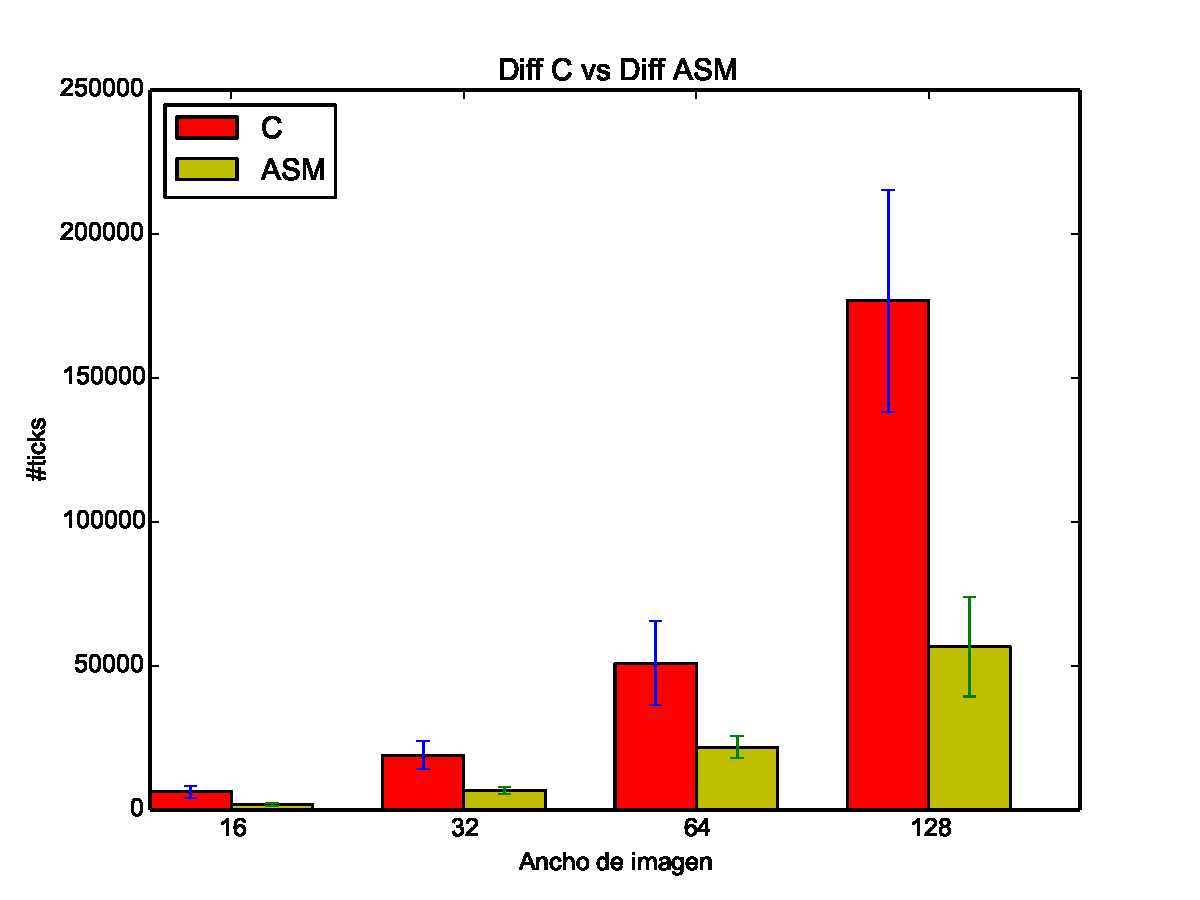
\includegraphics[width=1\textwidth]{../graficos/barplot_diff1}
  \caption{\footnotesize Cantidad de ticks de clock en función del ancho de la imagen (considerando imágenes cuadradas) para ambas implementaciones de diferencia. La altura de las barras es la media 0.25-podada de las muestras, mientras que las barras azules representan la varianza.}
  \label{fig:exp-diff-bar1}
\end{minipage}%
\hspace{0.03\textwidth}
\begin{minipage}{0.45\textwidth}   
  \centering
    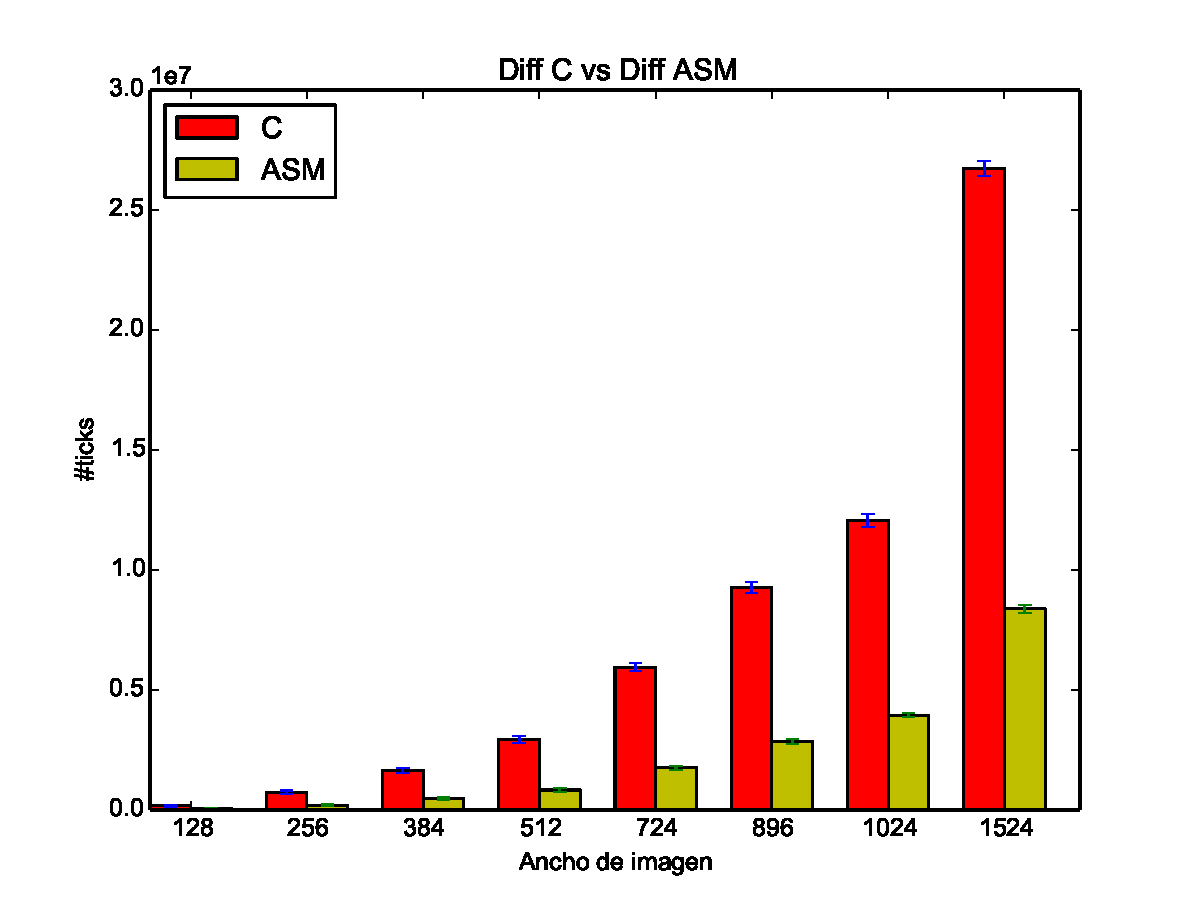
\includegraphics[width=1\textwidth]{../graficos/barplot_diff2} 
  \caption{\footnotesize Cantidad de ticks de clock en función del ancho de la imagen (considerando imágenes cuadradas) para ambas implementaciones de diferencia. La altura de las barras es la media 0.25-podada de las muestras, mientras que las barras azules representan la varianza.}
  \label{fig:exp-diff-bar2}
\end{minipage}%
\end{figure}

Ahora bien, si en lugar de graficar (en el eje de ordenadas) la cantidad de ticks del clock, normalizamos, es decir graficamos la cantidad de ciclos de clock por píxel, podemos obtener un gráfico de puntos como el que se observa en la figura \ref{fig:exp-diff-line}. Notemos que este gráfico nos permite ver varias cosas que se perdían en los gráficos anteriores. En primer término, vemos que ambas curvas de puntos tienen similar pendiente, aunque razonablemente ASM sigue siendo entre tres y cuatro veces más rapido en esta categoría. Esto nuevamente parece ser consecuencia de que ambas implementaciones usen algoritmos similares. 

También es interesante notar que a medida que aumentamos el tamaño de la imagen, la varianza tiende a disminuir y converger al valor esperado. Esto es razonable, pues para una imagen pequeña que se procesa rápido, un cambio en el contexto del sistema representa un aumento en el tiempo de cómputo mucho más significativo que para una imagen grande que tarda bastante en procesarse, lo que amortiza en algún punto estas diferencias.

Además, vemos que las curvas tienen dos etapas: una inicial, para los anchos hasta 128 píxeles, que decrece, es decir, que el tiempo de cómputo insumido por cada píxel (en promedio) es decreciente; la segunda etapa muestra una convergencia hacia un valor del eje de ordenadas. Pensemos a que puede deberse cada cosa.

Lo primero posiblemente sea consecuencia de lo rápido que se procesan imágenes de tamaño relativamente pequeño. Esta velocidad podría producir que los \emph{miss} tengan más peso, generando un menor \emph{hit-rate}, pues la cantidad de accesos a memoria que se hacen en total es relativamente chica para imágenes chicas. Así mismo, los cambios de contexto que se pudieran dar, pueden tomar un tiempo significativo en relación al tiempo que toma ejecutar cada iteración del filtro.

La convergencia que se muestra en la segunda etapa puede pensarse como el producto de que el \emph{diff} varía linealmente con respecto al tamaño de la imagen (esto es cuadráticamente respecto del ancho). Dicho de otra forma, si a una imagen de $m\times n$, se le agregan 4 píxeles (por poner un ejemplo) más a cada una de las $m$ filas, esto implica que el \emph{diff\_c} va a tener que hacer 4 iteraciones más por cada una de ellas, mientras el \emph{diff\_asm} va a hacer sólo una más. Pero el tiempo de cómputo que agrega procesar cada uno de estos píxeles es el mismo que aportaba un píxel de la imagen vieja (llamémoslo $t_{pixelViejo}$), pues asumimos que la imagen ya era lo bastante grande como para que el efecto de la cache o los cambios de contexto al agrandar más la imagen no sean significativos, por lo que al dividir el tiempo total por la nueva cantidad de píxeles obtenemos el mismo tiempo por pixel que antes (aproximadamente, claro esta). Es decir, que 
\begin{equation}
\label{eq:convergencia1}
	\begin{split}
	t_{pixelNuevo} & = \frac{ t_{totalViejo} + m \times 4 \times t_{pixelViejo}}{m\times (n+4)} \\
				   & = \frac{ (m\times n) \times t_{pixelViejo} + m \times 4 \times t_{pixelViejo}}{m\times (n+4)} \\
				   & = \frac{ (m\times n + m \times 4) \times t_{pixelViejo}}{m\times (n+4)} \\
				   & = \frac{ m\times (n + 4) \times t_{pixelViejo}}{m\times (n+4)} \\
				   & = t_{pixelViejo} 
	\end{split}
\end{equation}

Claramente, en la ecuación (\ref{eq:convergencia1}) podemos cambiar 4 por cualquier múltiplo y sigue funcionando.
\begin{figure}
 	\centering
 	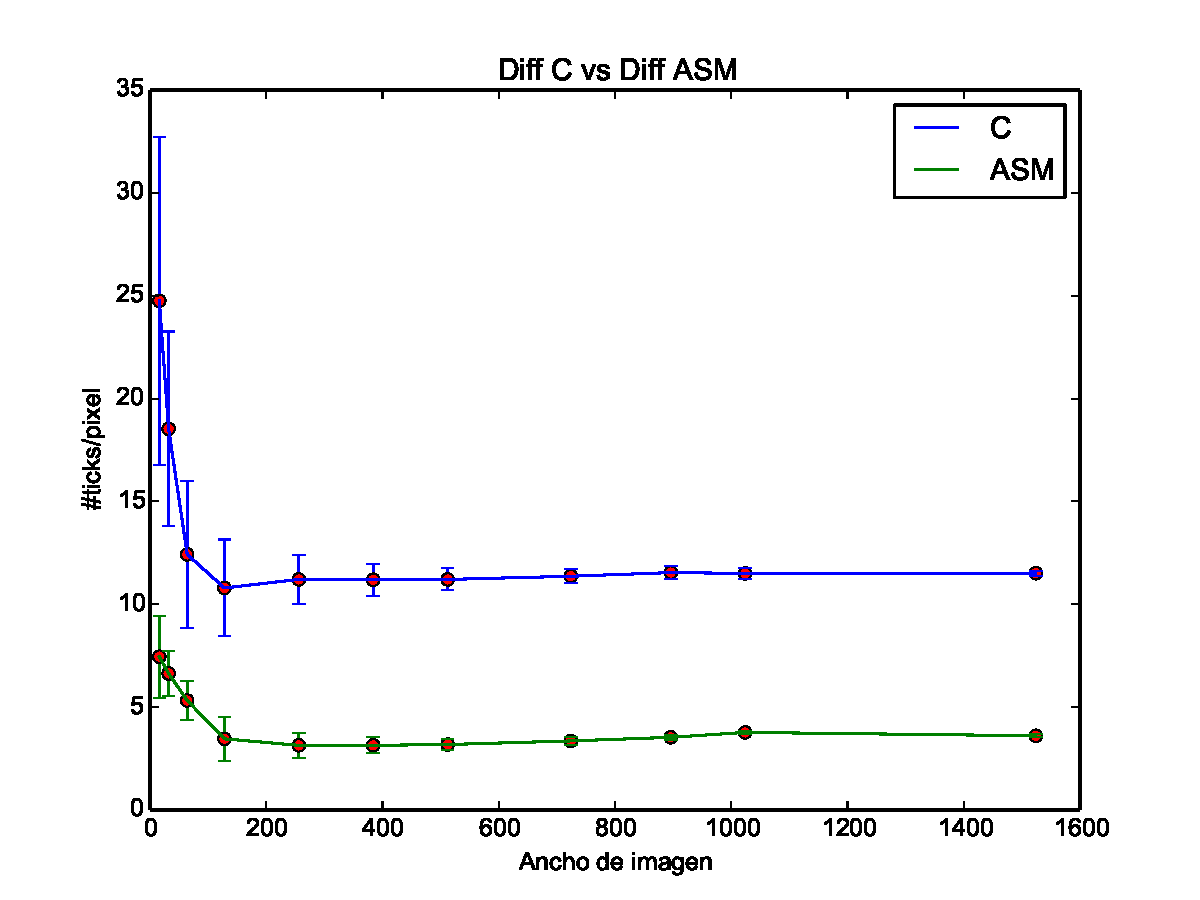
\includegraphics[width=0.75\textwidth]{../graficos/diff_gcc.pdf}
	\caption{\footnotesize Gráfico que muestra la cantidad de ticks de reloj por pixel que se requieren para aplicar el filtro de diferencias implementado en C y en assembler en función del ancho de la imagen. Todas las imágenes son cuadradas y fueron generadas pseudo-aleatoriamente. Los puntos rojos representan la media 0.25-podada calculada sobre las muestras obtenidas, mientras que los segmentos verticales indican la desviación standard.}
	\label{fig:exp-diff-line}
\end{figure}

\paragraph*{Experimentos blur}
Pasemos ahora a analizar los resultados correspondientes a blur.

\begin{figure}[H]
 	\centering
 	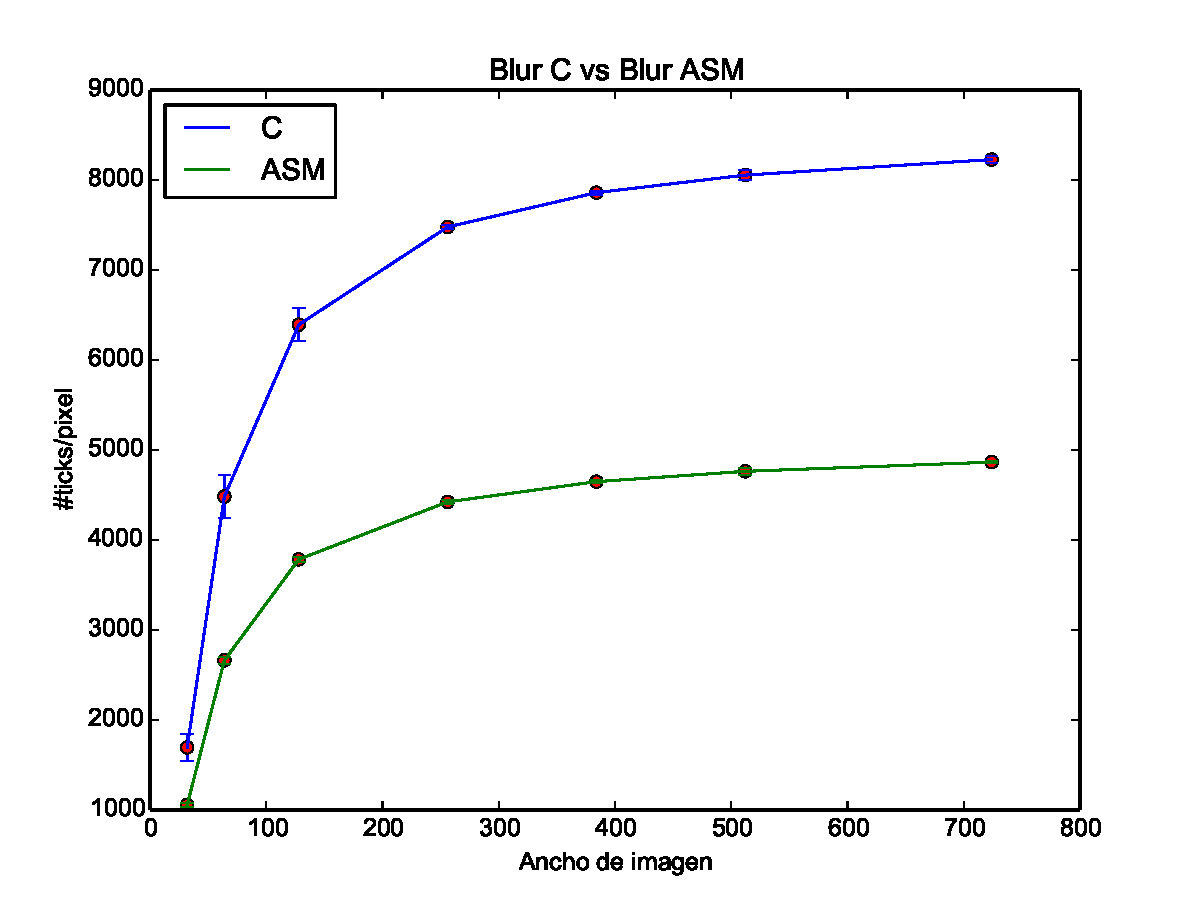
\includegraphics[width=0.75\textwidth]{../graficos/blur_v2_lineplot_3-9.pdf}
	\caption{\footnotesize Gráfico que muestra la cantidad de ticks de reloj por pixel que se requieren para aplicar el filtro de blur gaussiano implementado en C y en assembler en función del ancho de la imagen, para $\sigma = 3$, $radio = 9$. Todas las imágenes son cuadradas y fueron generadas pseudo-aleatoriamente. Los puntos rojos representan la media 0.25-podada calculada sobre las muestras obtenidas, mientras que los segmentos verticales indican la desviación standard.}
	\label{fig:exp-blur1}
\end{figure}

La figura \ref{fig:exp-blur1} nos muestra los resultados obtenidos del experimento \ref{itm:exp-blur1}. En este caso consideramos directamente la versión normalizada, pues nos muestra claramente toda la información que necesitamos. Nuevamente, vemos que el tiempo de cómputo de las versiones en C y ASM varían con una curva de similar pendiente, pero la versión aprovecha el procesamiento SIMD sigue ganando gracias a la mejora en las constantes. No obstante podemos apreciar que en este caso la mejoría fue menor a la esperada: mientras que suponíamos una disminución de entre 2 y 3 veces en el tiempo de procesamiento, en la práctica sólo fue de entre 1.5 a 2 veces. Esto puede pensarse que es debido al alto grado de optimización que implica compilar el código en C con O3.

En este caso, como los tiempos de procesamiento de blur son mucho más altos que \emph{diff}, no apreciamos una primera etapa de decrecimiento en la curva, pues no se dan las condiciones explicadas antes. Lo que si es notable es que la curva lejos de ser constante como en \emph{diff} presenta un crecimiento logarítmico. Tratemos de ver porque pasa esto haciendo un análisis similar al hecho para el filtro de diferencias. En ese caso teníamos que el crecimiento era lineal en el tamaño de la imagen pues \emph{diff} sólo tabaja con un pixel en cada iteración de la versión C \footnote{Usamos esta que es más simple de explicar, pero todo es análogo a ASM.}. Sin embargo con el blur entra en consideración el radio, que es 9 en el caso del experimento. Por lo tanto, si tenemos una imagen y le agregamos más píxeles, por cada uno de ellos se nos suma una iteración adicional, pero dentro de la misma tenemos que operar con los 360 vecinos ($(2\times radio + 1)^2= 361$ incluyendo al píxel sobre el que estamos parados) del pixel que queremos procesar, más . Luego, por cada píxel que le agreguemos a la imagen estaremos agregando también 360 accesos a memoria para obtener los vecinos, y otros 361 para obtener los coeficientes del \emph{kernel}. Visto esto, es claro que el aumento en los píxeles no compensa el aumento en las operaciones (como si pasaba con $diff$) por lo que la cantidad de ciclos de clock por píxel va a aumentar indefectiblemente. No obstante, como el aumento de las operaciones por píxel es constante ocurre que cada aumento impacta cada vez menos en el tiempo total de procesado, por lo que pasado cierto punto, la curva tiende a variar cada vez menos y converger hacia un valor del eje de ordenadas, lo que genera que tenga una forma logarítmica.


\begin{figure}[H]
 	\centering
 	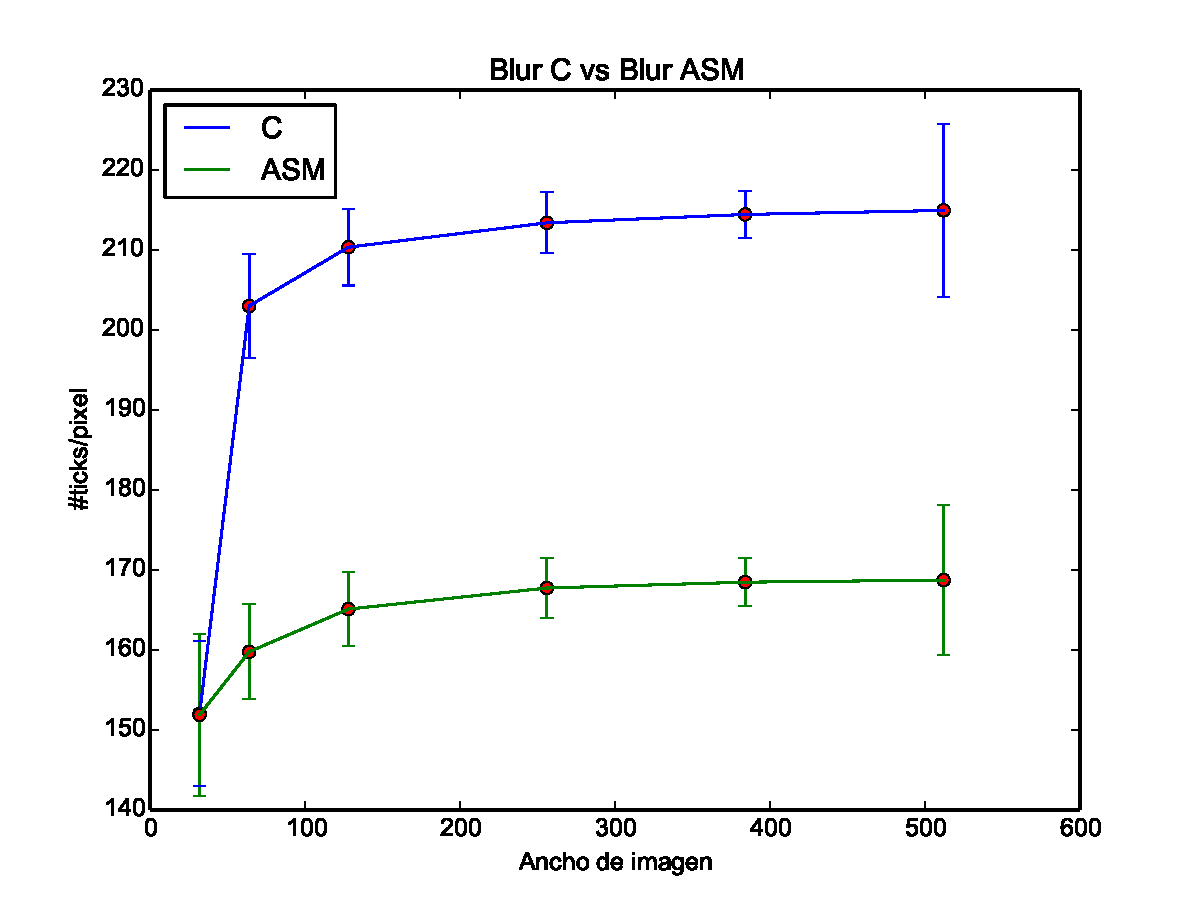
\includegraphics[width=0.75\textwidth]{../graficos/blur_v2_lineplot_03-1.pdf}
	\caption{\footnotesize Gráfico que muestra la cantidad de ticks de reloj por pixel que se requieren para aplicar el filtro de blur gaussiano implementado en C y en assembler en función del ancho de la imagen, para $\sigma = 0.3$, $radio = 1$ Todas las imágenes son cuadradas y fueron generadas pseudo-aleatoriamente. Los puntos rojos representan la media 0.25-podada calculada sobre las muestras obtenidas, mientras que los segmentos verticales indican la desviación standard.}
	\label{fig:exp-blur2}
\end{figure}

Si ahora analizamos la figura \ref{fig:exp-blur2} correspondiente al experimento \ref{itm:exp-blur2}, vemos que nuevamente obtenemos curvas logarítmicas, pero con una diferencia importante: las pendientes de las curvas son mucho más suaves. Esto efectivamente se debe a que redujimos el valor del radio de 9 a 1, por lo que que la cantidad de accesos a memoria que se realizan por píxel es de 8 para los vecinos, y 9 para los elementos del \emph{kernel}. Esto lógicamente genera que la velocidad de cambio de la curva sea menor.

\begin{figure}[H]
 	\centering
 	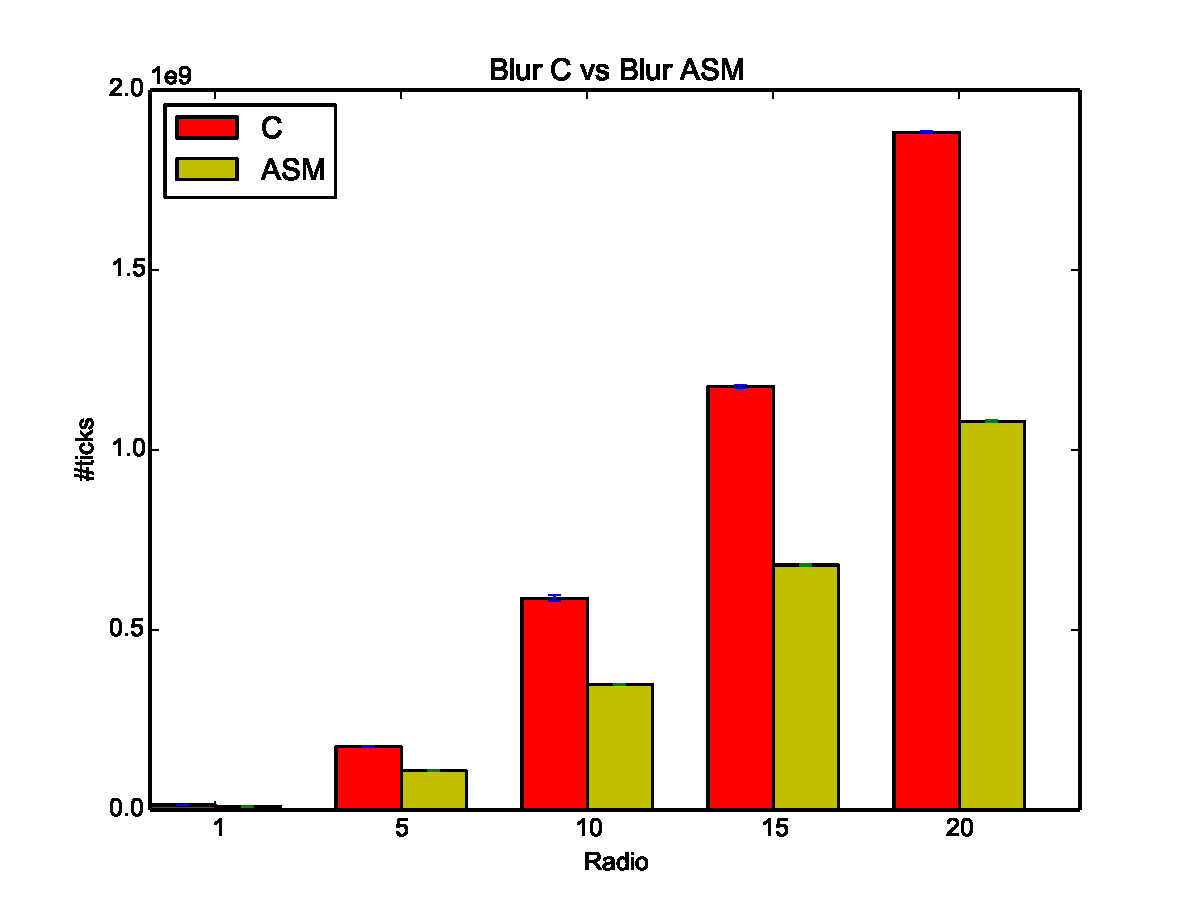
\includegraphics[width=0.75\textwidth]{../graficos/barplot_radio.pdf}
	\caption{\footnotesize Gráfico que muestra la cantidad de ticks de reloj en función del radio, para una imagen de 256x256}
	\label{fig:exp-blur3}
\end{figure}

La figura \ref{fig:exp-blur3} muestra que al variar sólo el radio, C y ASM varían sus performances de forma similar.

\begin{figure}[H]
 	\centering
 	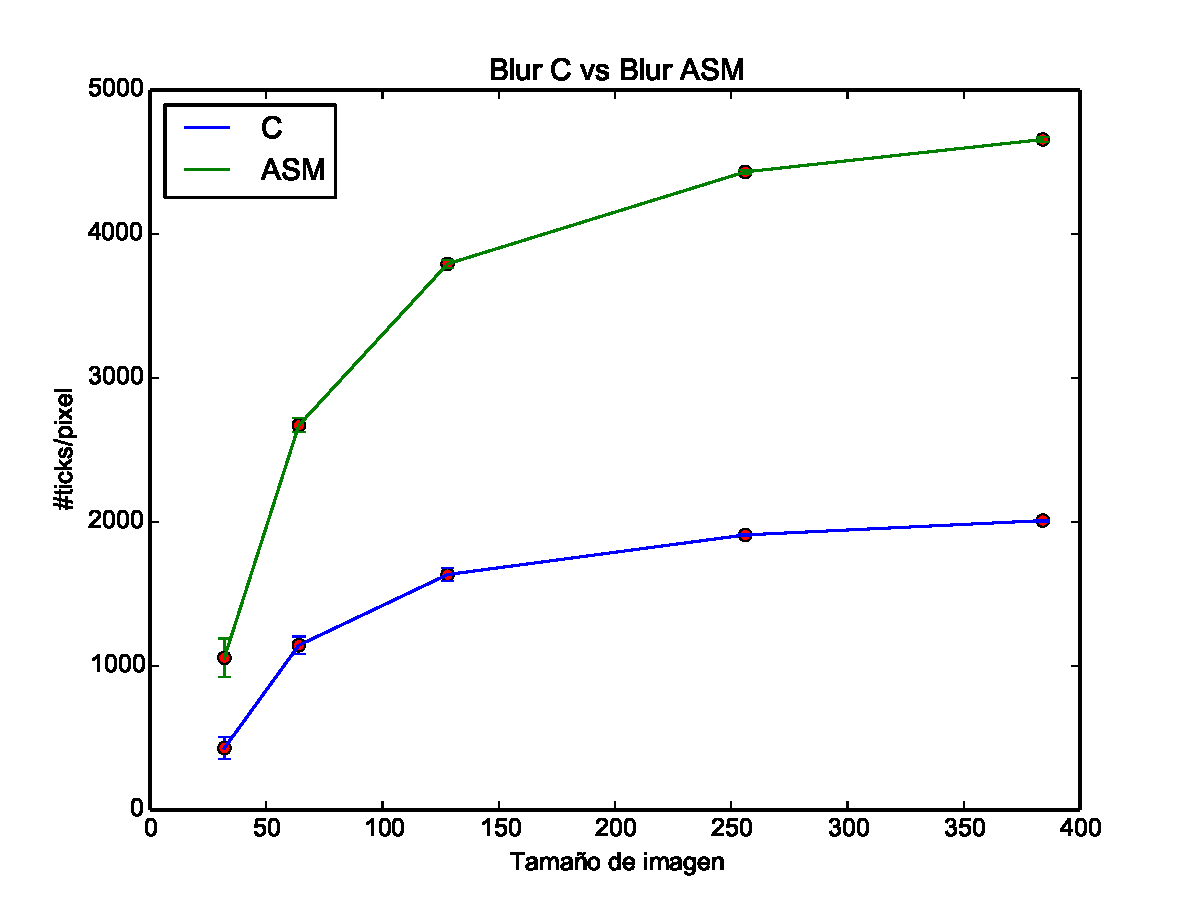
\includegraphics[width=0.75\textwidth]{../graficos/blur_v1_lineplot.pdf}
	\caption{\footnotesize Gráfico que muestra la cantidad de ticks de reloj por pixel que se requieren para aplicar el filtro de blur gaussiano implementado en C y en assembler en función del ancho de la imagen, para $\sigma = 3$, $radio = 9$ Todas las imágenes son cuadradas y fueron generadas pseudo-aleatoriamente. Los puntos rojos representan la media 0.25-podada calculada sobre las muestras obtenidas, mientras que los segmentos verticales indican la desviación standard.}
	\label{fig:exp-blur4}
\end{figure}

%Posibles experimentos:
% *Para blur: fijar el sigma, y hacer un lineplot en función del radio